\section{FaBoの使い方}
\subsection{FaBoの接続}
このの授業ではFaBoのシールドとFaBoのブリックを使います。FaBoはセンサーとRaspberry Piを簡単につなぐことができるよう、あらかじめ配線がされています。

\begin{figure}[htbp]
  \begin{minipage}[b]{0.45\linewidth}
    \centering
    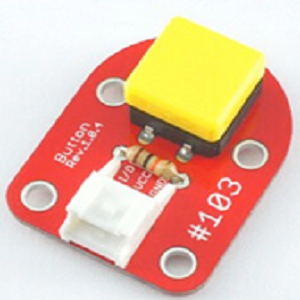
\includegraphics[keepaspectratio, scale=0.6]{images/chap05/text05-img028.png}
    \caption{デジタル信号の例}
    \label{fig4}
  \end{minipage}
  \begin{minipage}[b]{0.45\linewidth}
    \centering
    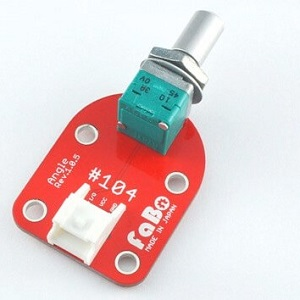
\includegraphics[keepaspectratio, scale=0.6]{images/chap05/text05-img022.jpg}
    \caption{アナログ信号の例}
    \label{fig5}
  \end{minipage}
\end{figure}

LEDは電池で動きますが、FaBoブリックはRaspberry Piを電源として動きます。FaBoでないセンサーは、電源のプラスとマイナス、センサーの出力などを考えて、Raspberry Piに繋ぎます。しかし、FaBoのシールドとブリックは必要な配線が統一されているため、自分でどのように線を繋ぐかを考えなくても簡単に使えます。
それでは、早速FaBoを使ってみましょう。

\begin{itembox}[c]{\Large\textcolor{red}{注意!}}
  FaboのシールドをRaspberry Piとつなげるときは、必ずRaspberry Piをシャットダウンして電源を切りましょう。
\end{itembox}

% \begin{enumerate}
%   \item Raspberry Piの電源を切ります。\\
%   \item ケーブルを使用して、FaBoのシールドをRaspberry Piとつなげます。この時、なるべくシールドをまっすぐに押しこむようにしましょう。ピン(金属の棒の部分)を曲げないように注意してください。シールドにもトゲのある所があるのでケガをしないように注意しましょう。\\
%   \begin{figure}[H]
%     \centering
%     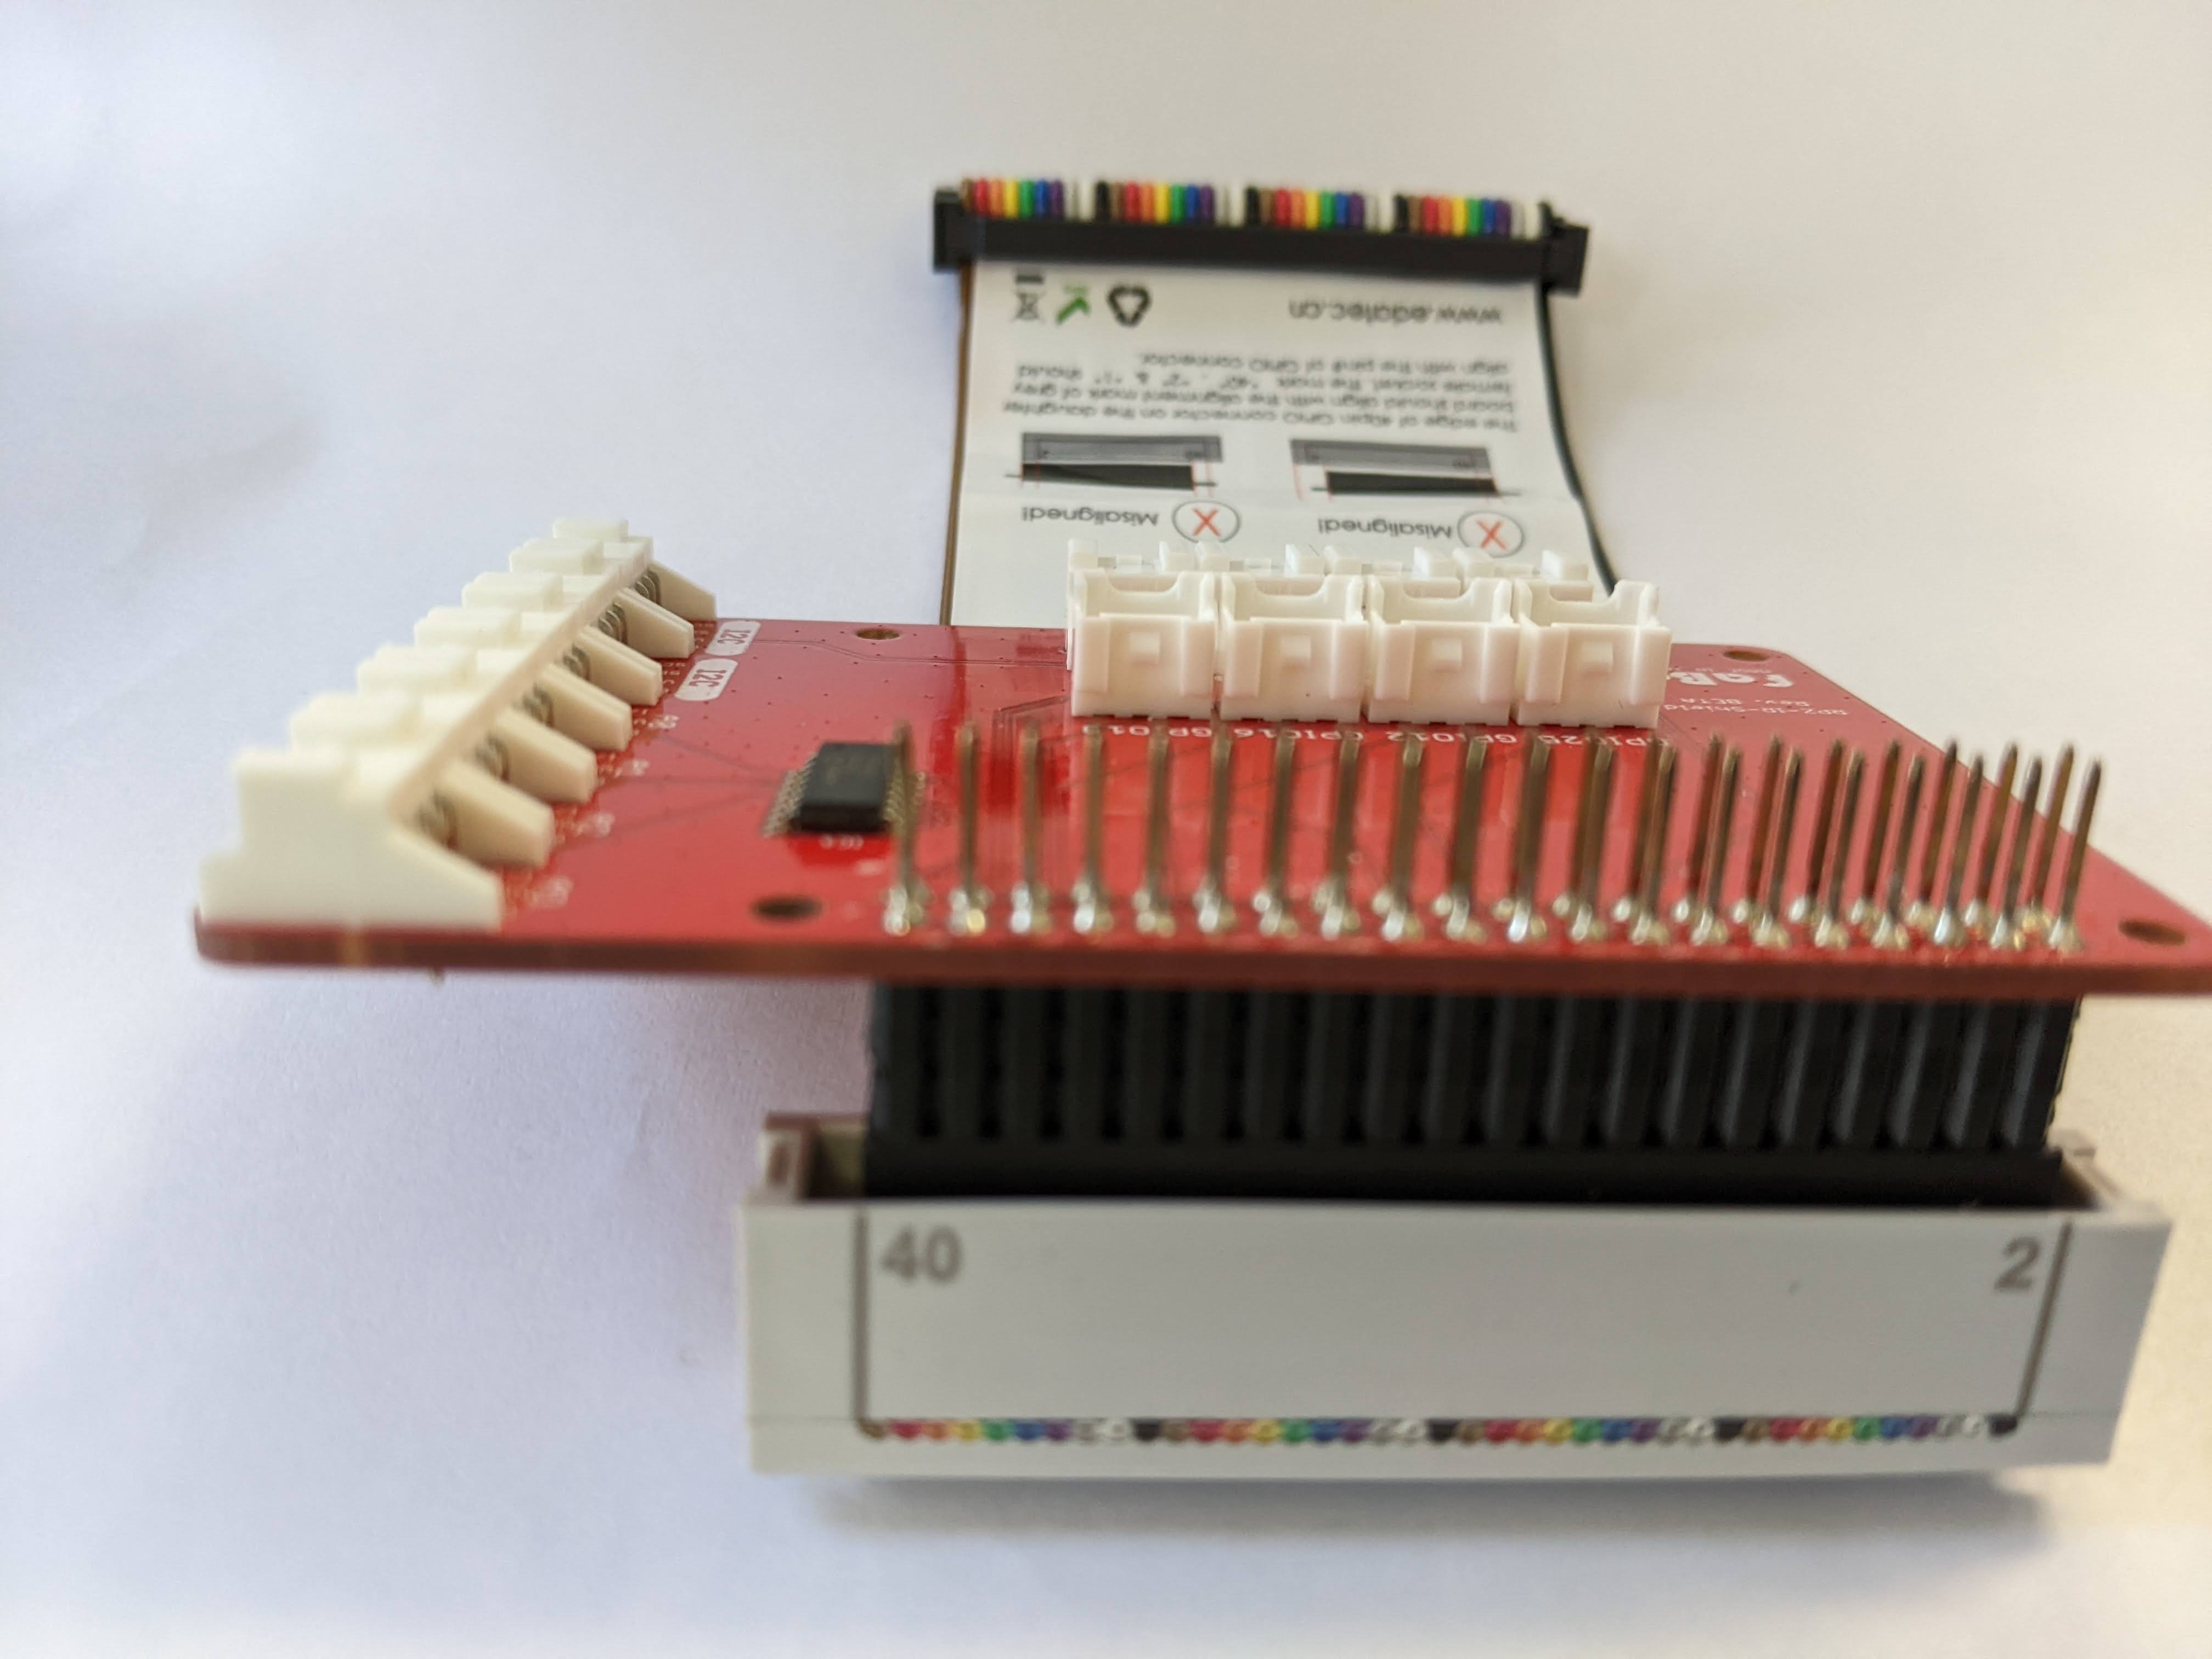
\includegraphics[width=\hsize/2]{images/chap05/fabo_and_cable_rearview.jpg}
%     \caption{FaBoのシールドとケーブルの\ruby{接続}{せつ|ぞく} (後ろから見た図)}
%   \end{figure}
%   \begin{figure}[H]
%     \centering
%     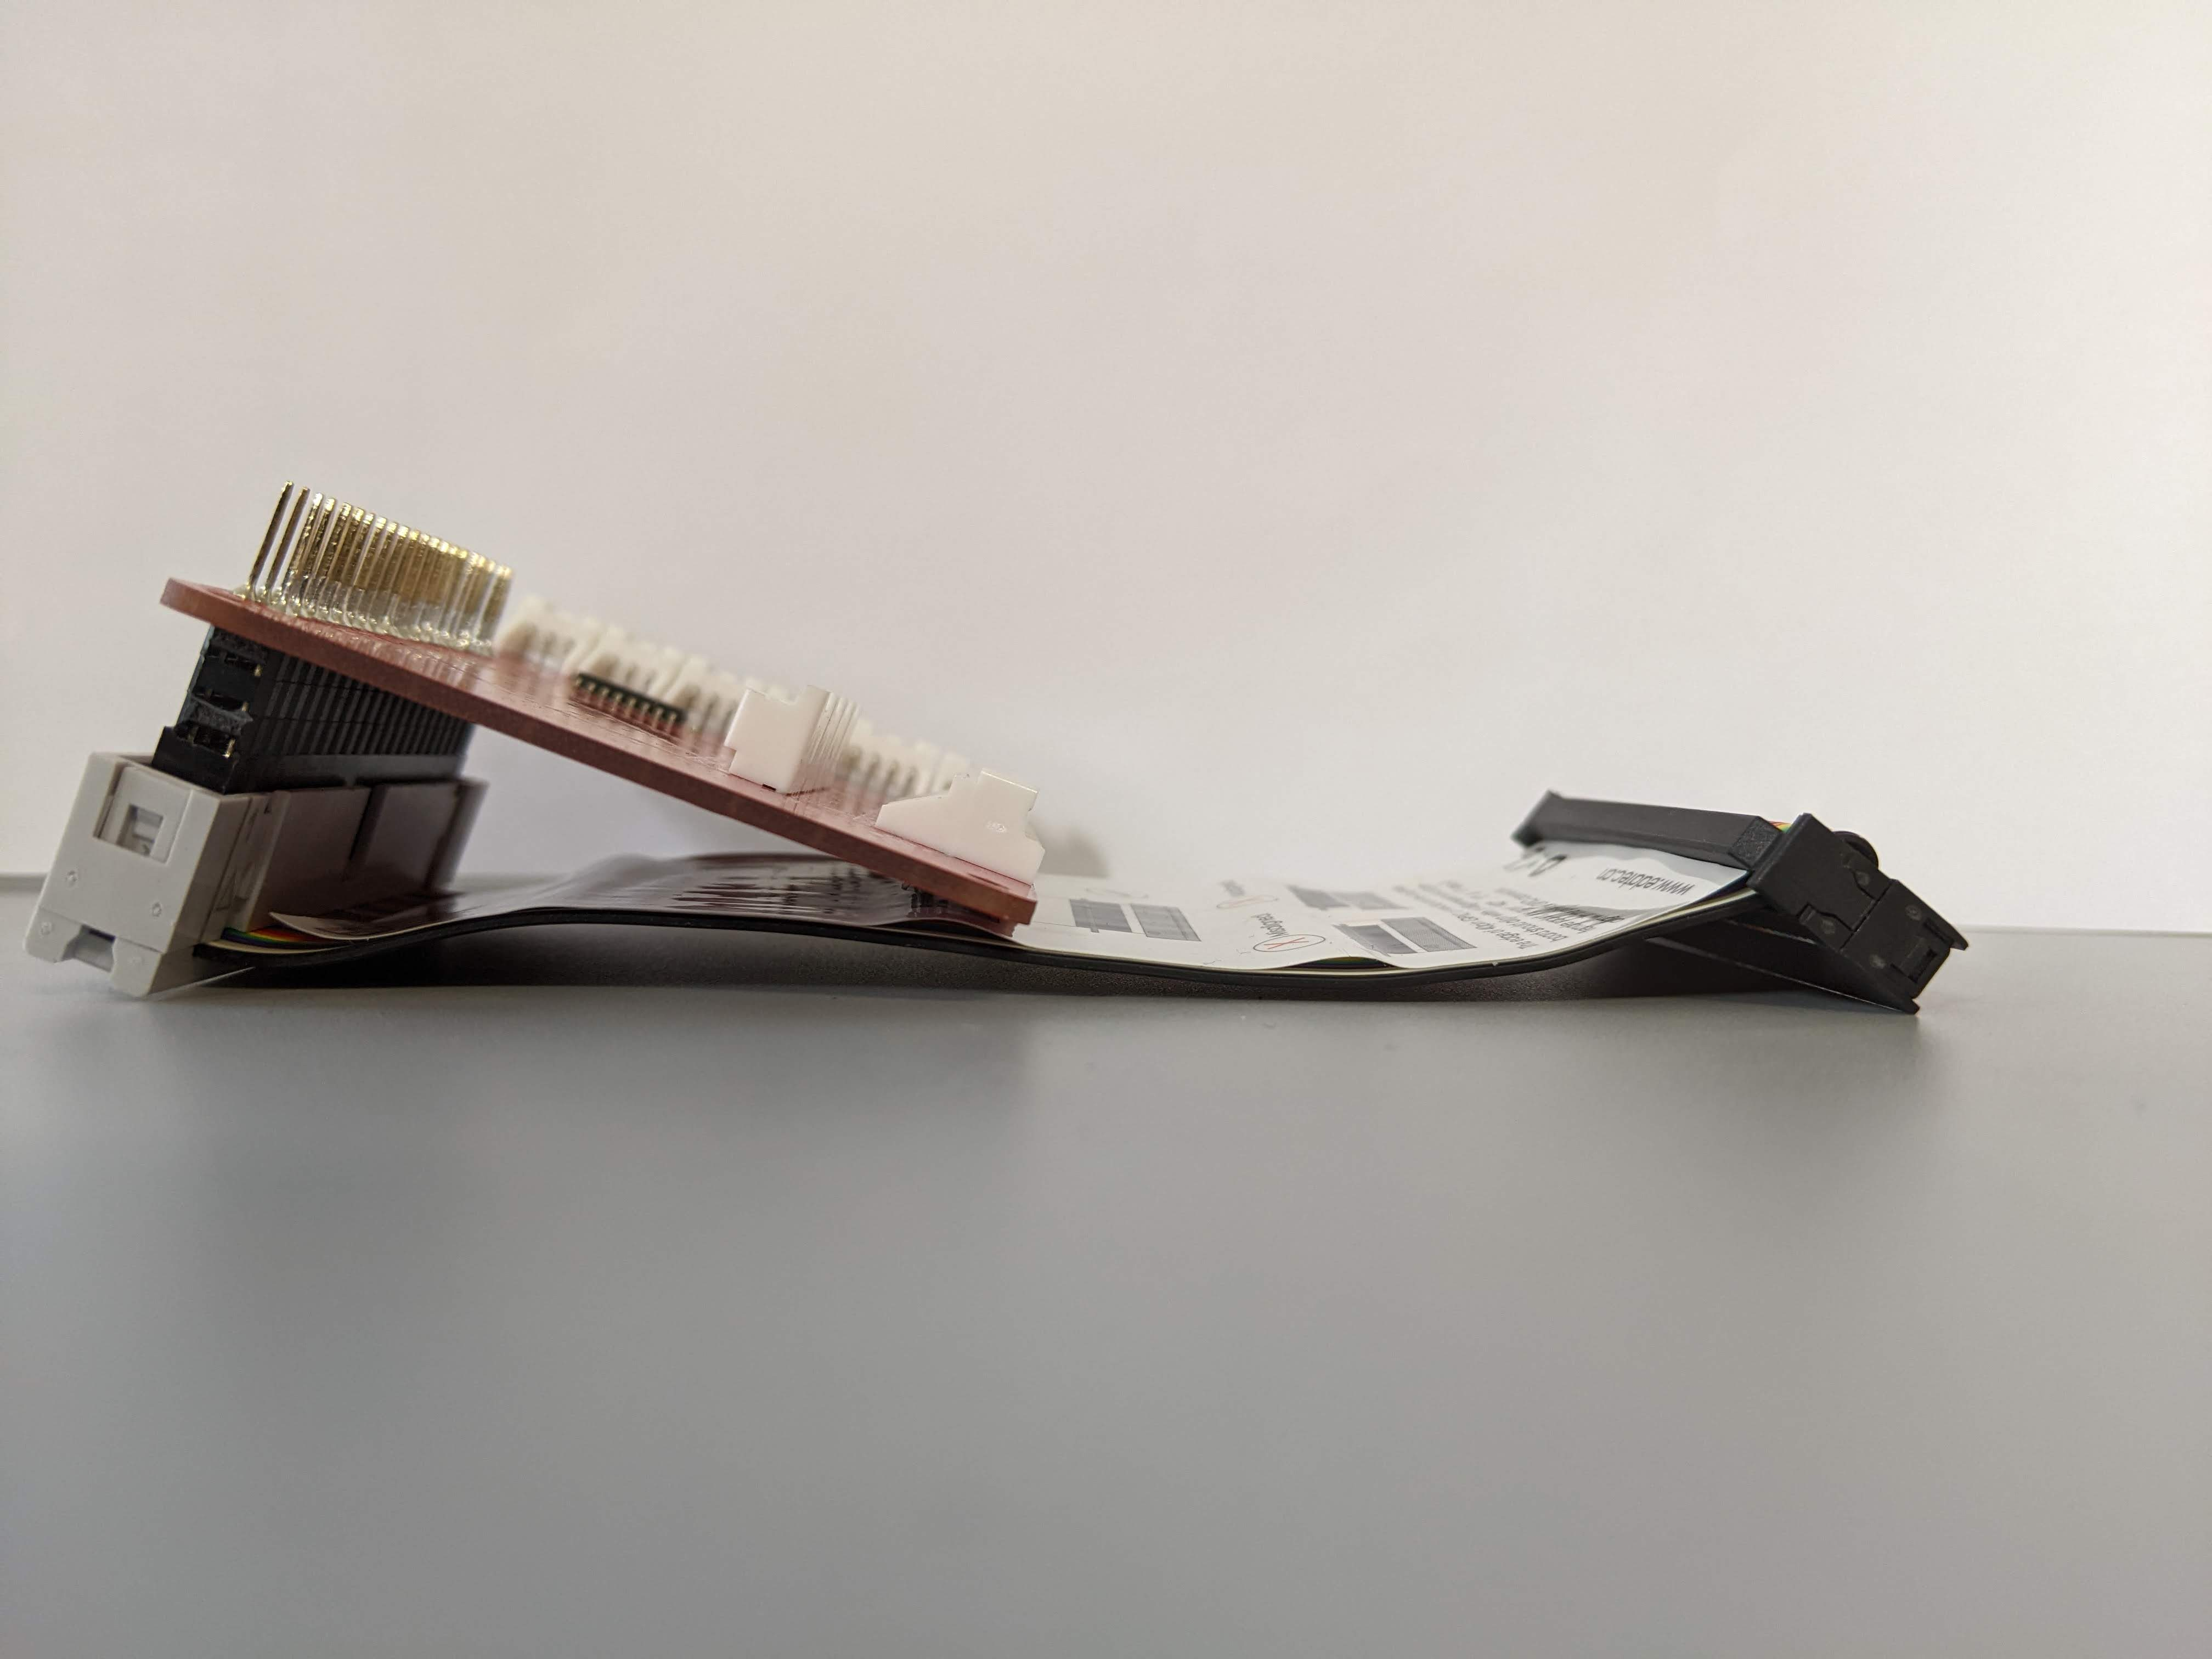
\includegraphics[width=\hsize/2]{images/chap05/fabo_and_cable_sideview.png}
%     \caption{FaBoのシールドとケーブルの\ruby{接続}{せつ|ぞく} (\ruby{横}{よこ}から見た図)}
%   \end{figure}
%   \begin{figure}[H]
%     \centering
%     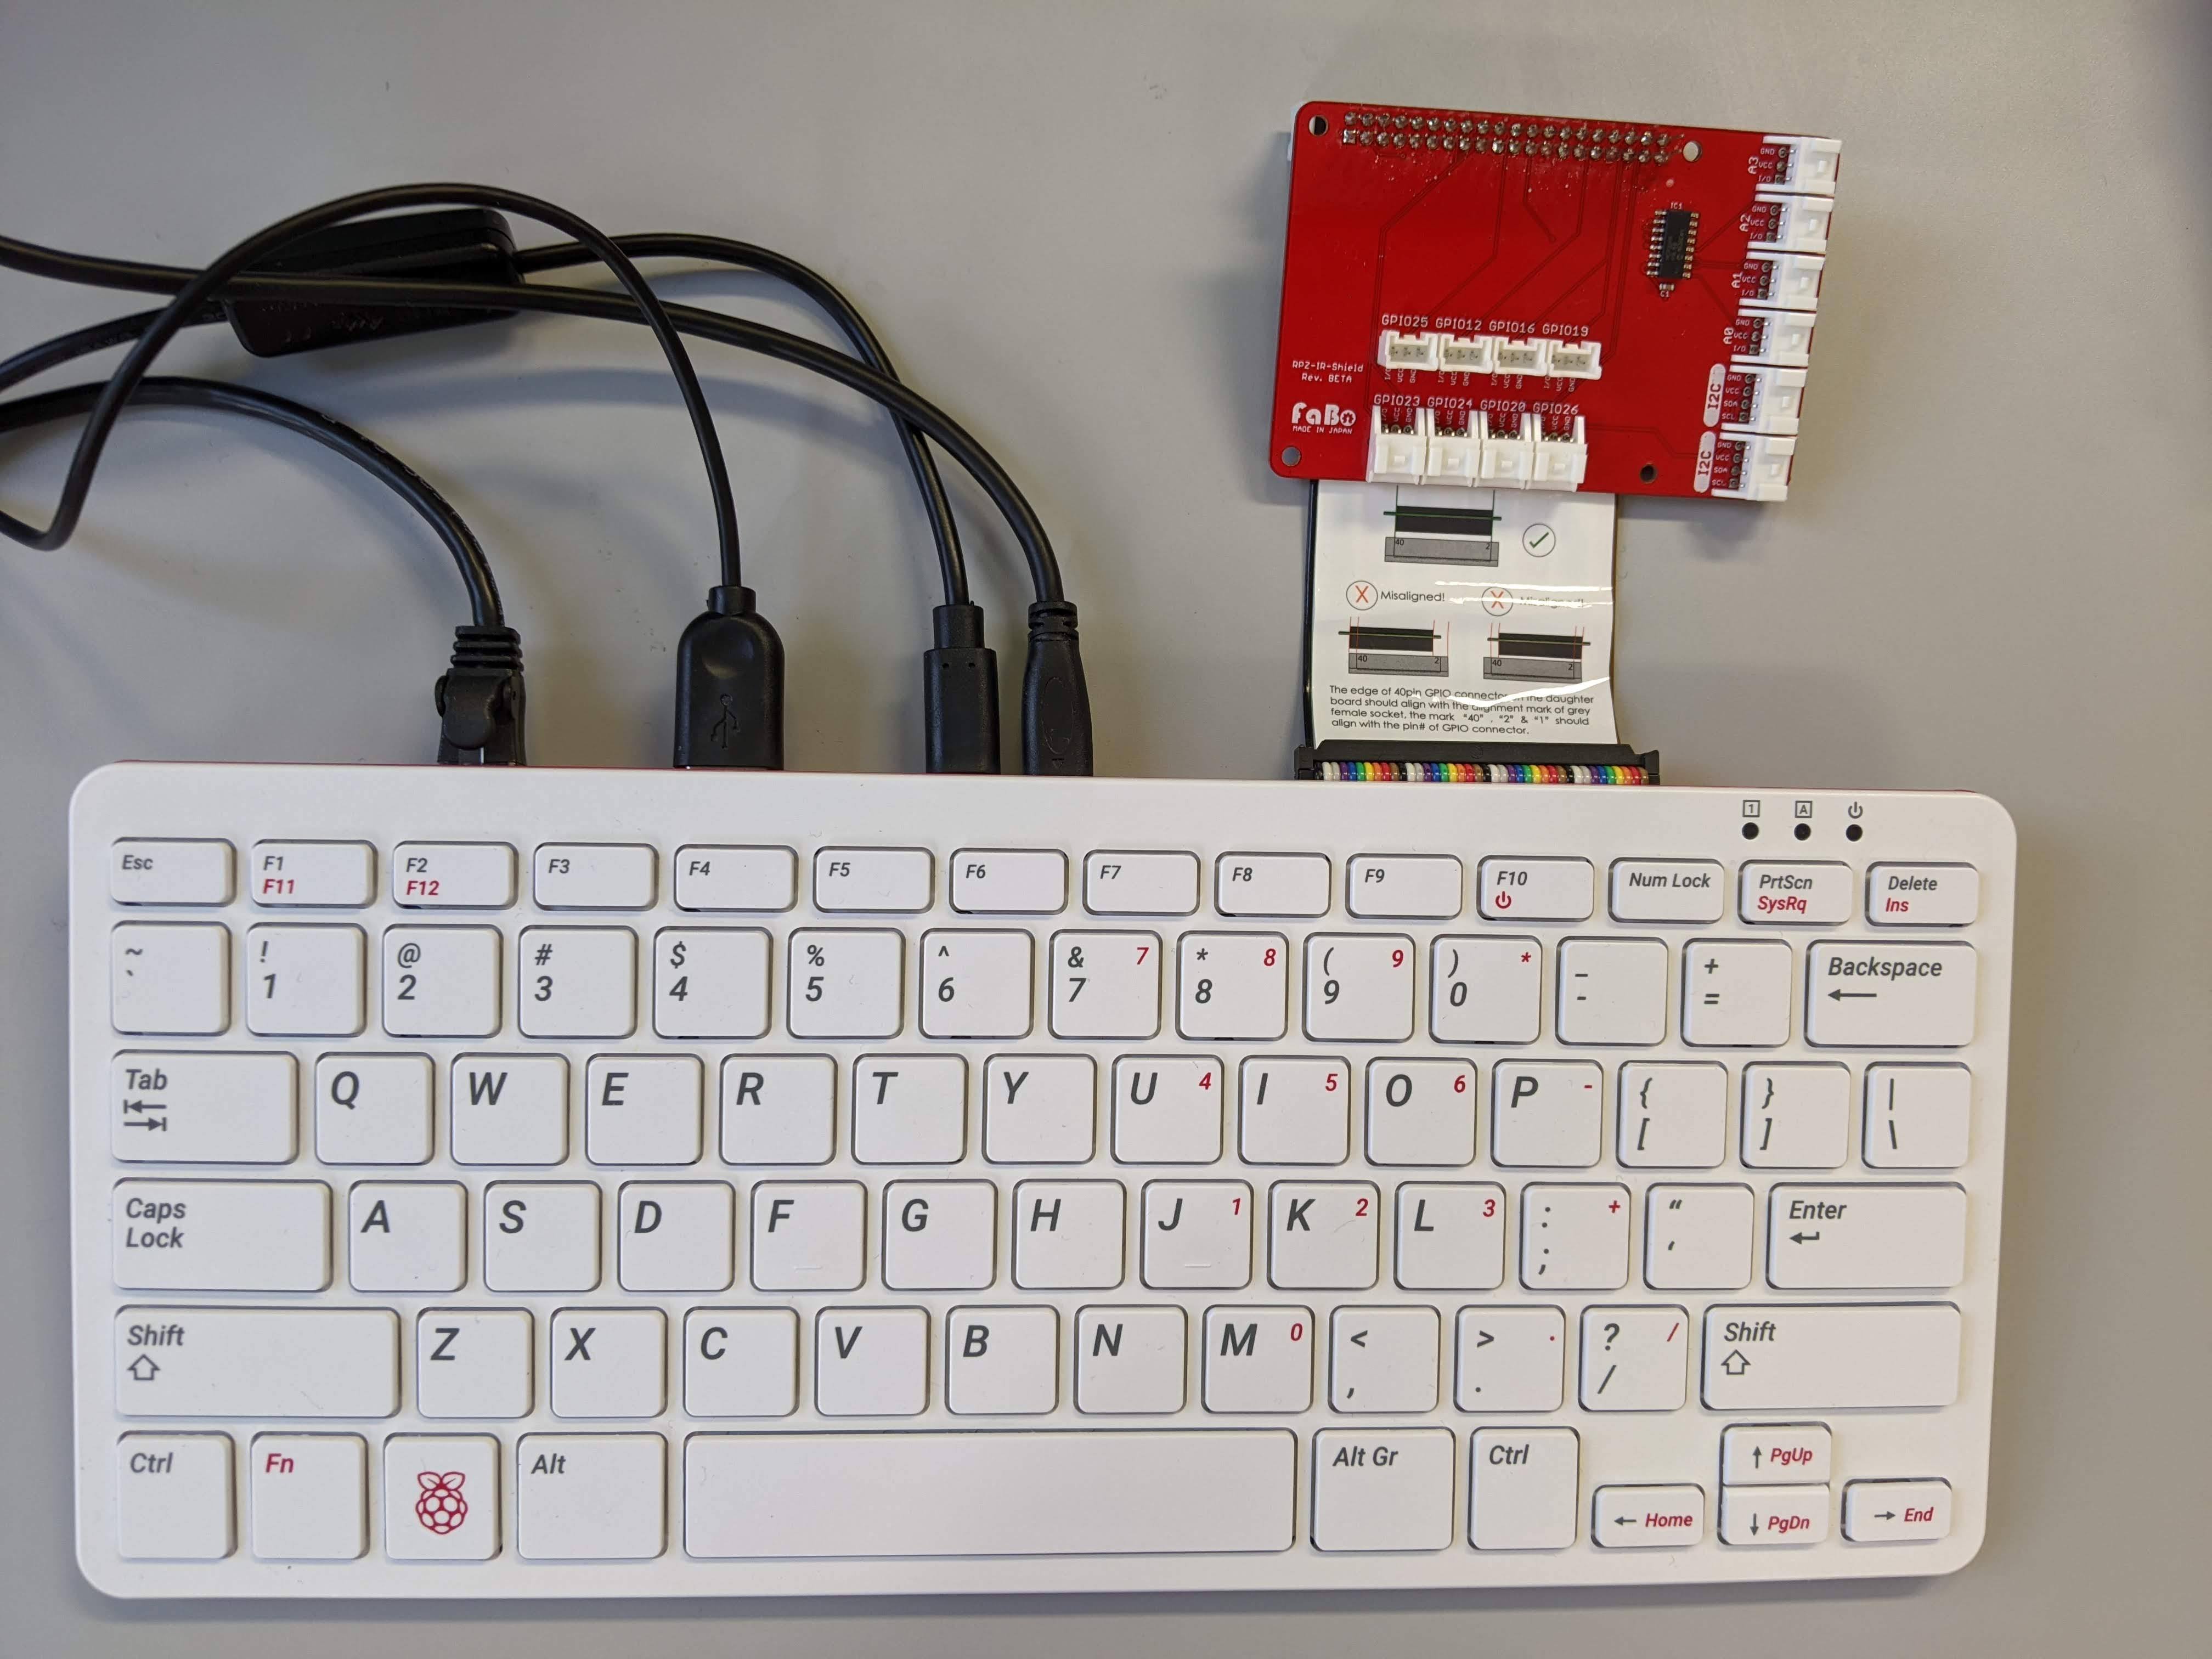
\includegraphics[width=\hsize/2]{images/chap05/fabo_connected_to_rpi400.jpg}
%     \caption{FaBoのシールドとRaspberry Piの\ruby{接続}{せつ|ぞく}}
%   \end{figure}
%   \item 同様にして、センサーボードをFaBoのシールドの上につなげます。\\
%   \begin{figure}[H]
%     \centering
%     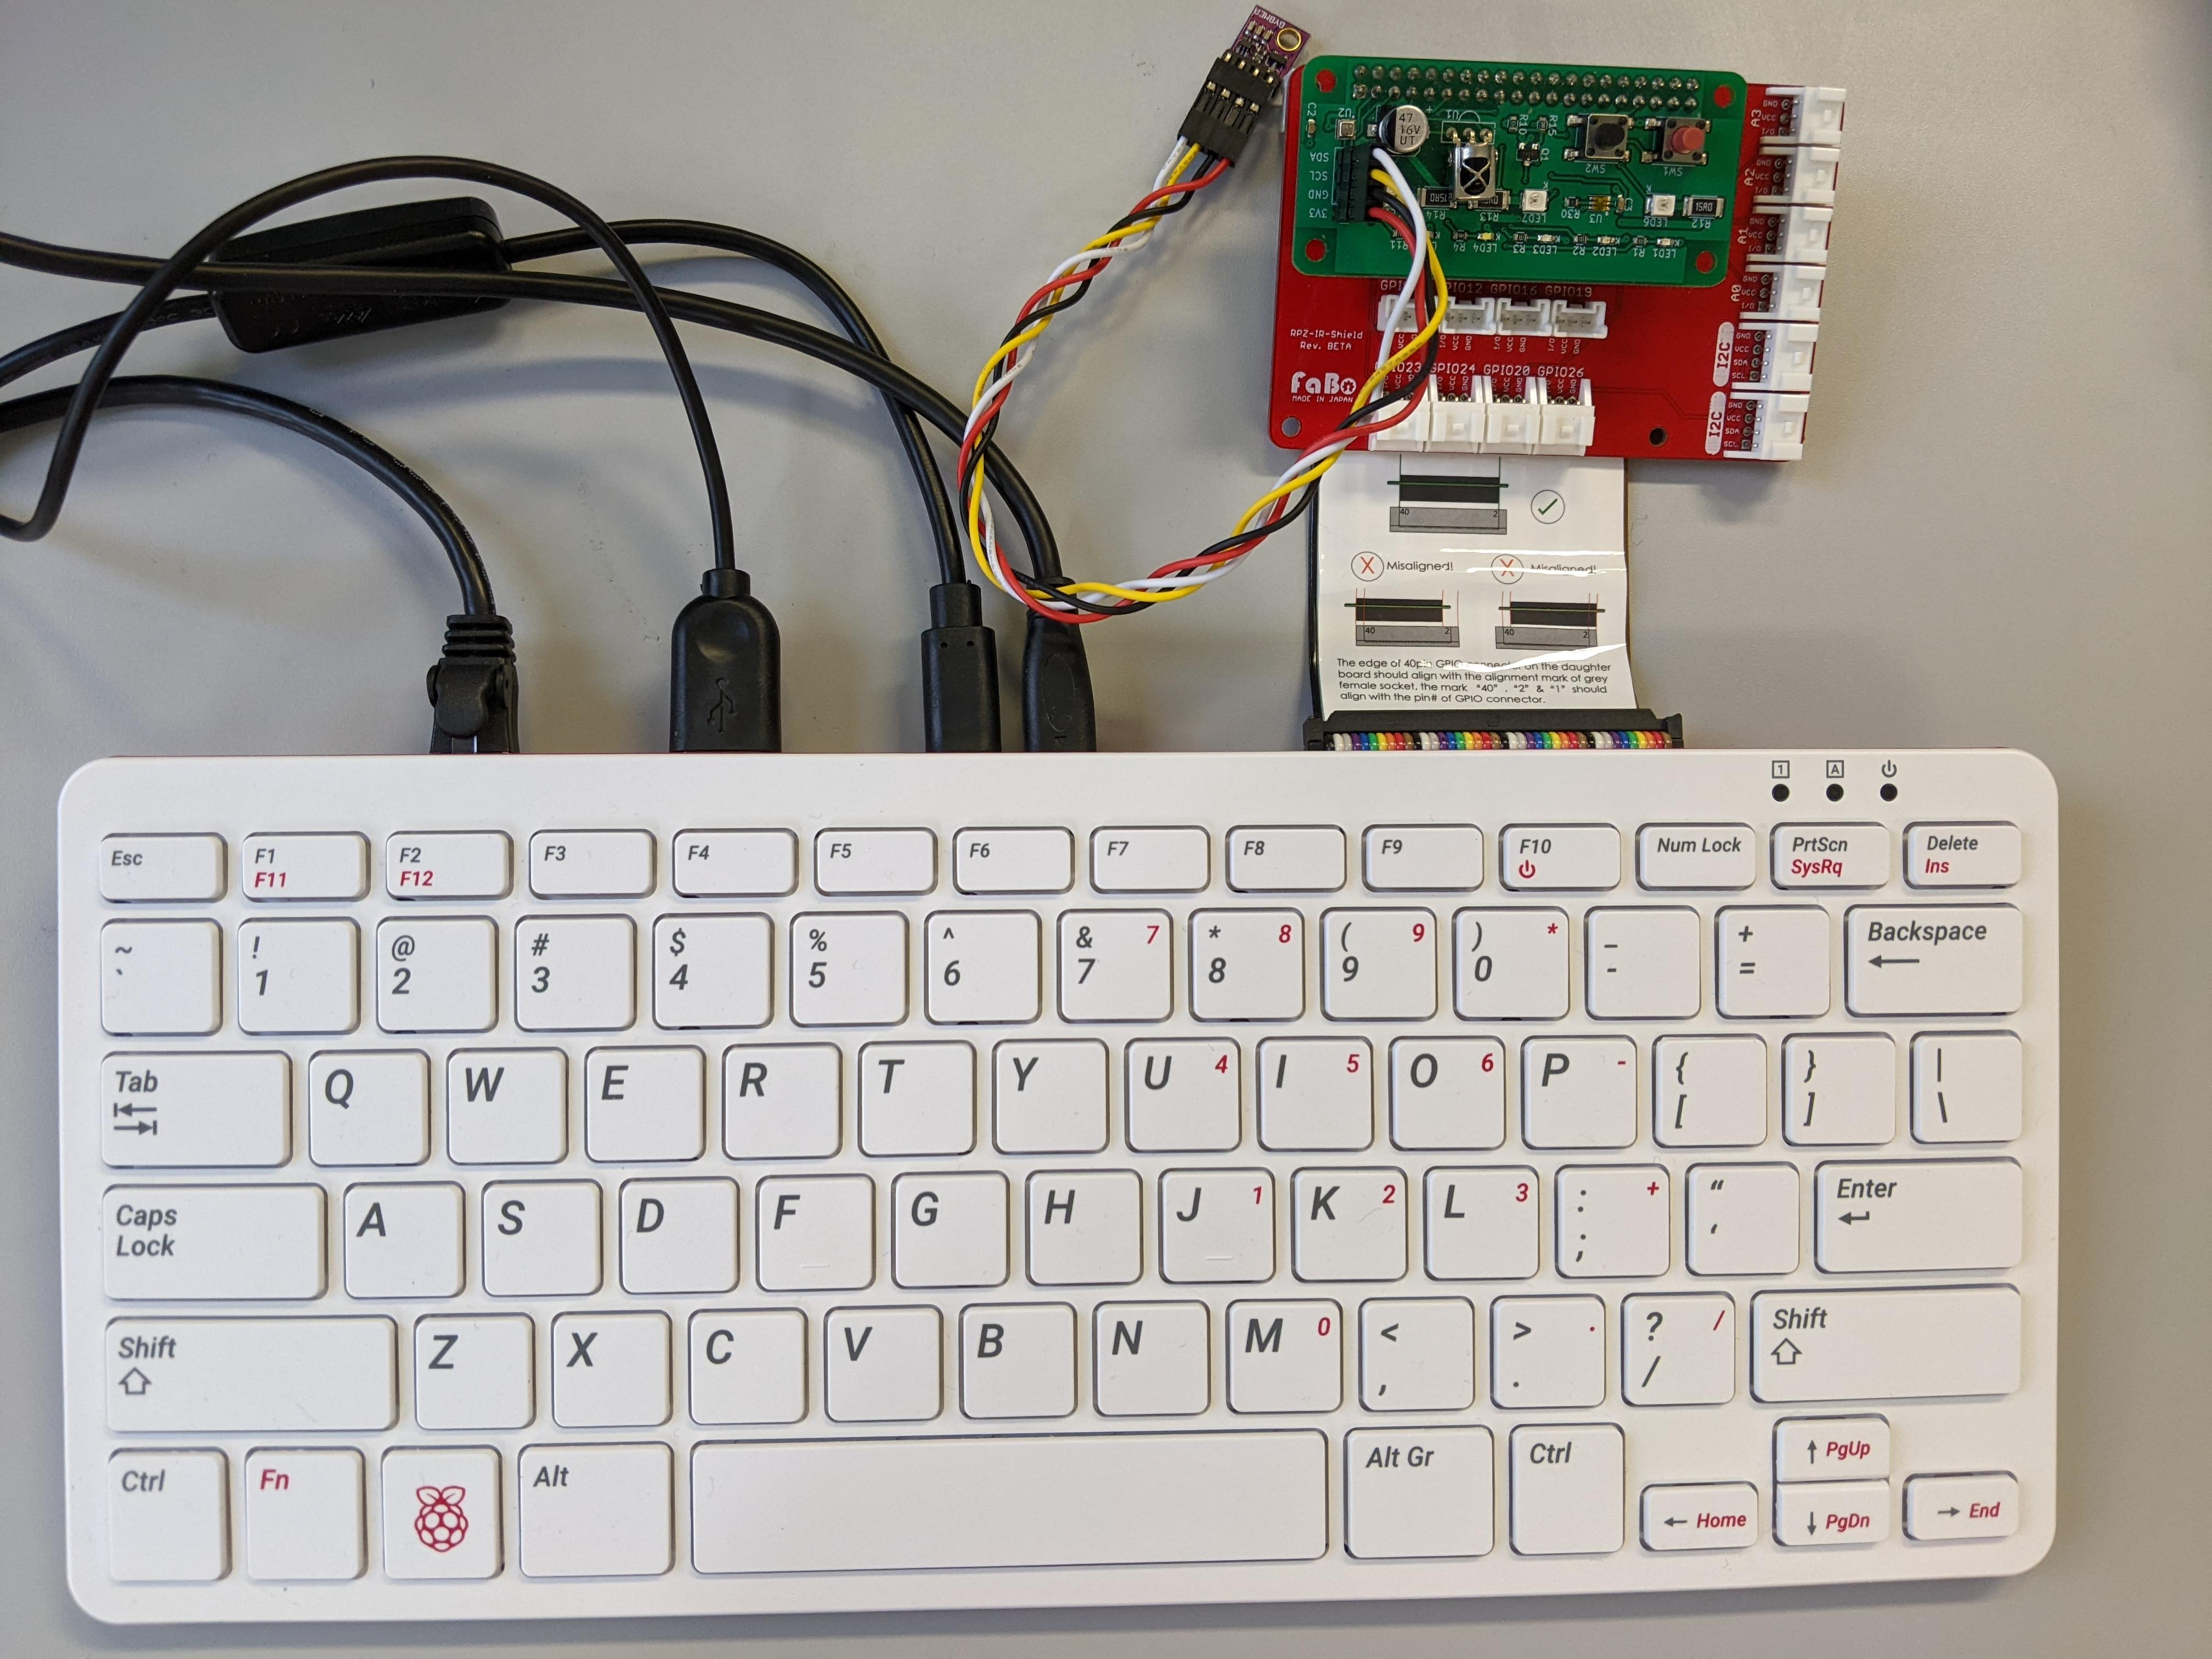
\includegraphics[width=\hsize/2]{images/chap05/sb_on_fabo_connected_to_rpi400.jpg}
%     \caption{センサーボードとFaBoのシールドの接続}
%   \end{figure}
%   \item LEDをケーブルとつなげましょう。奥までコネクタを押しこんでください。\\
%   \begin{figure}[H]
%     \centering
%     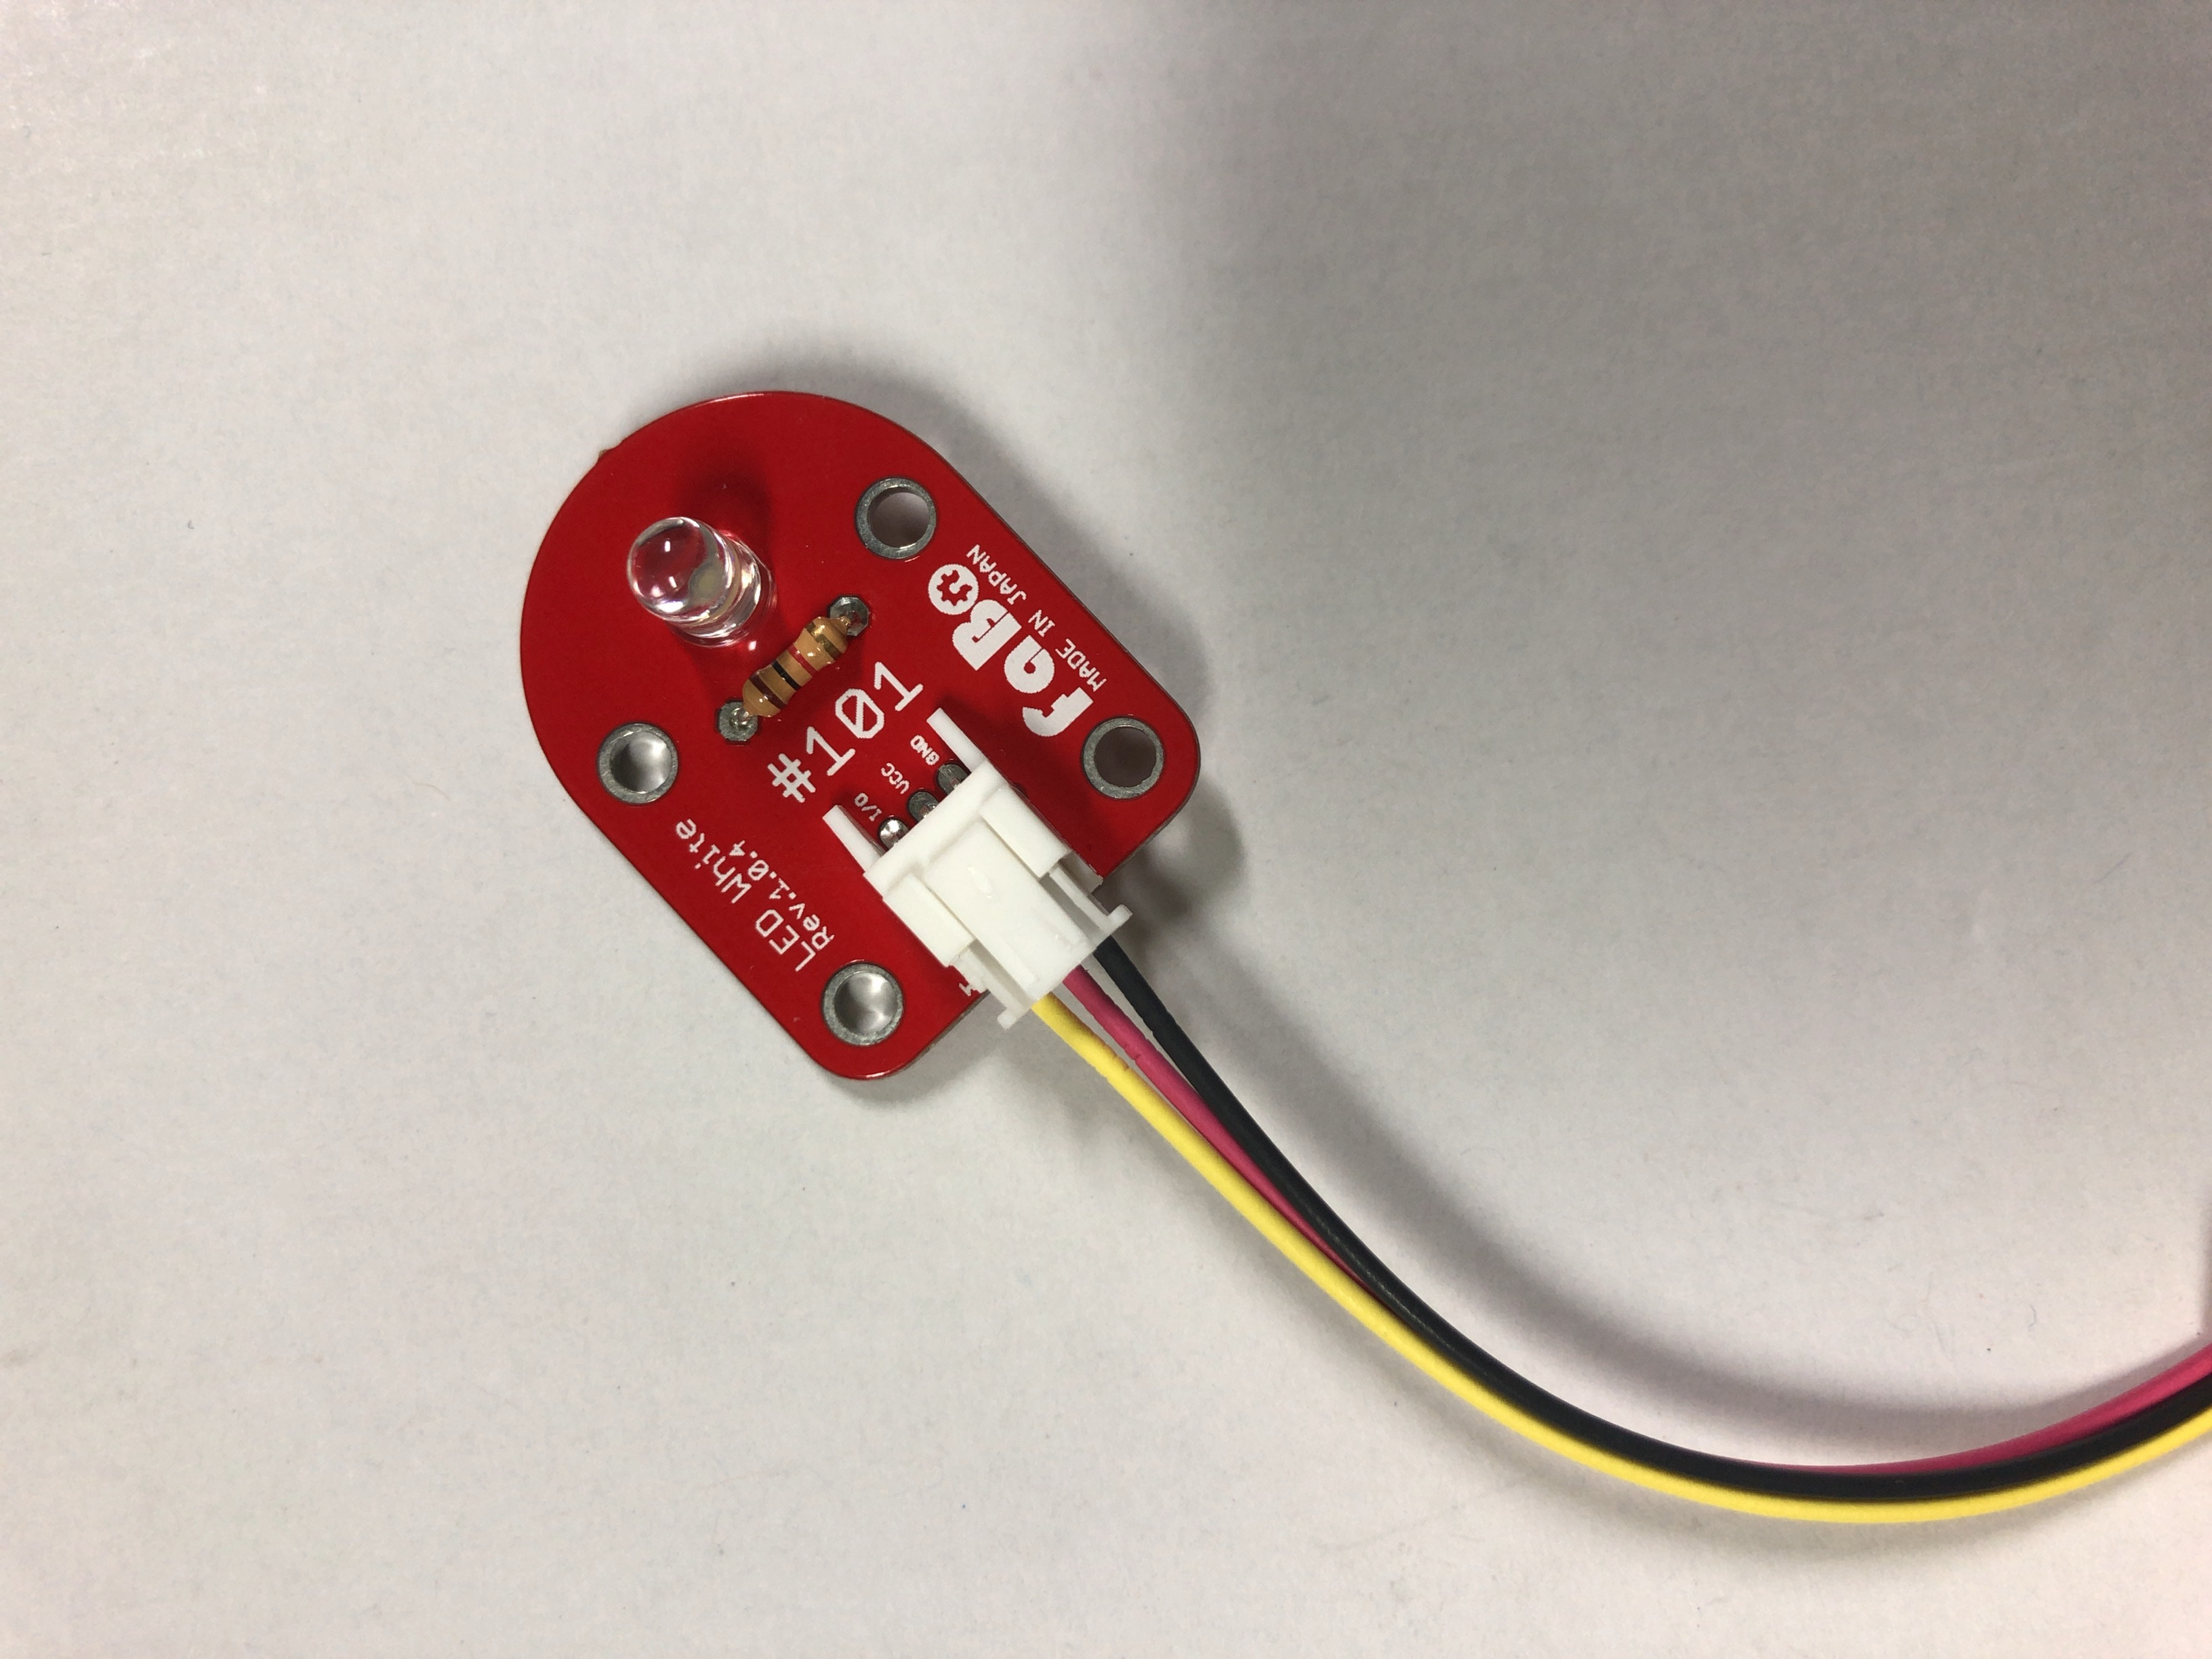
\includegraphics[width=\hsize/2]{images/chap05/text05-img008.jpg}
%     \caption{Faboのブリックとケーブルの接続}
%   \end{figure}
%   \item シールドとケーブルをつなげましょう。今回はGPIO23のところにつなげます。このときも奥までコネクタを押しこんでください。\\
%   \begin{figure}[H]
%     \centering
%     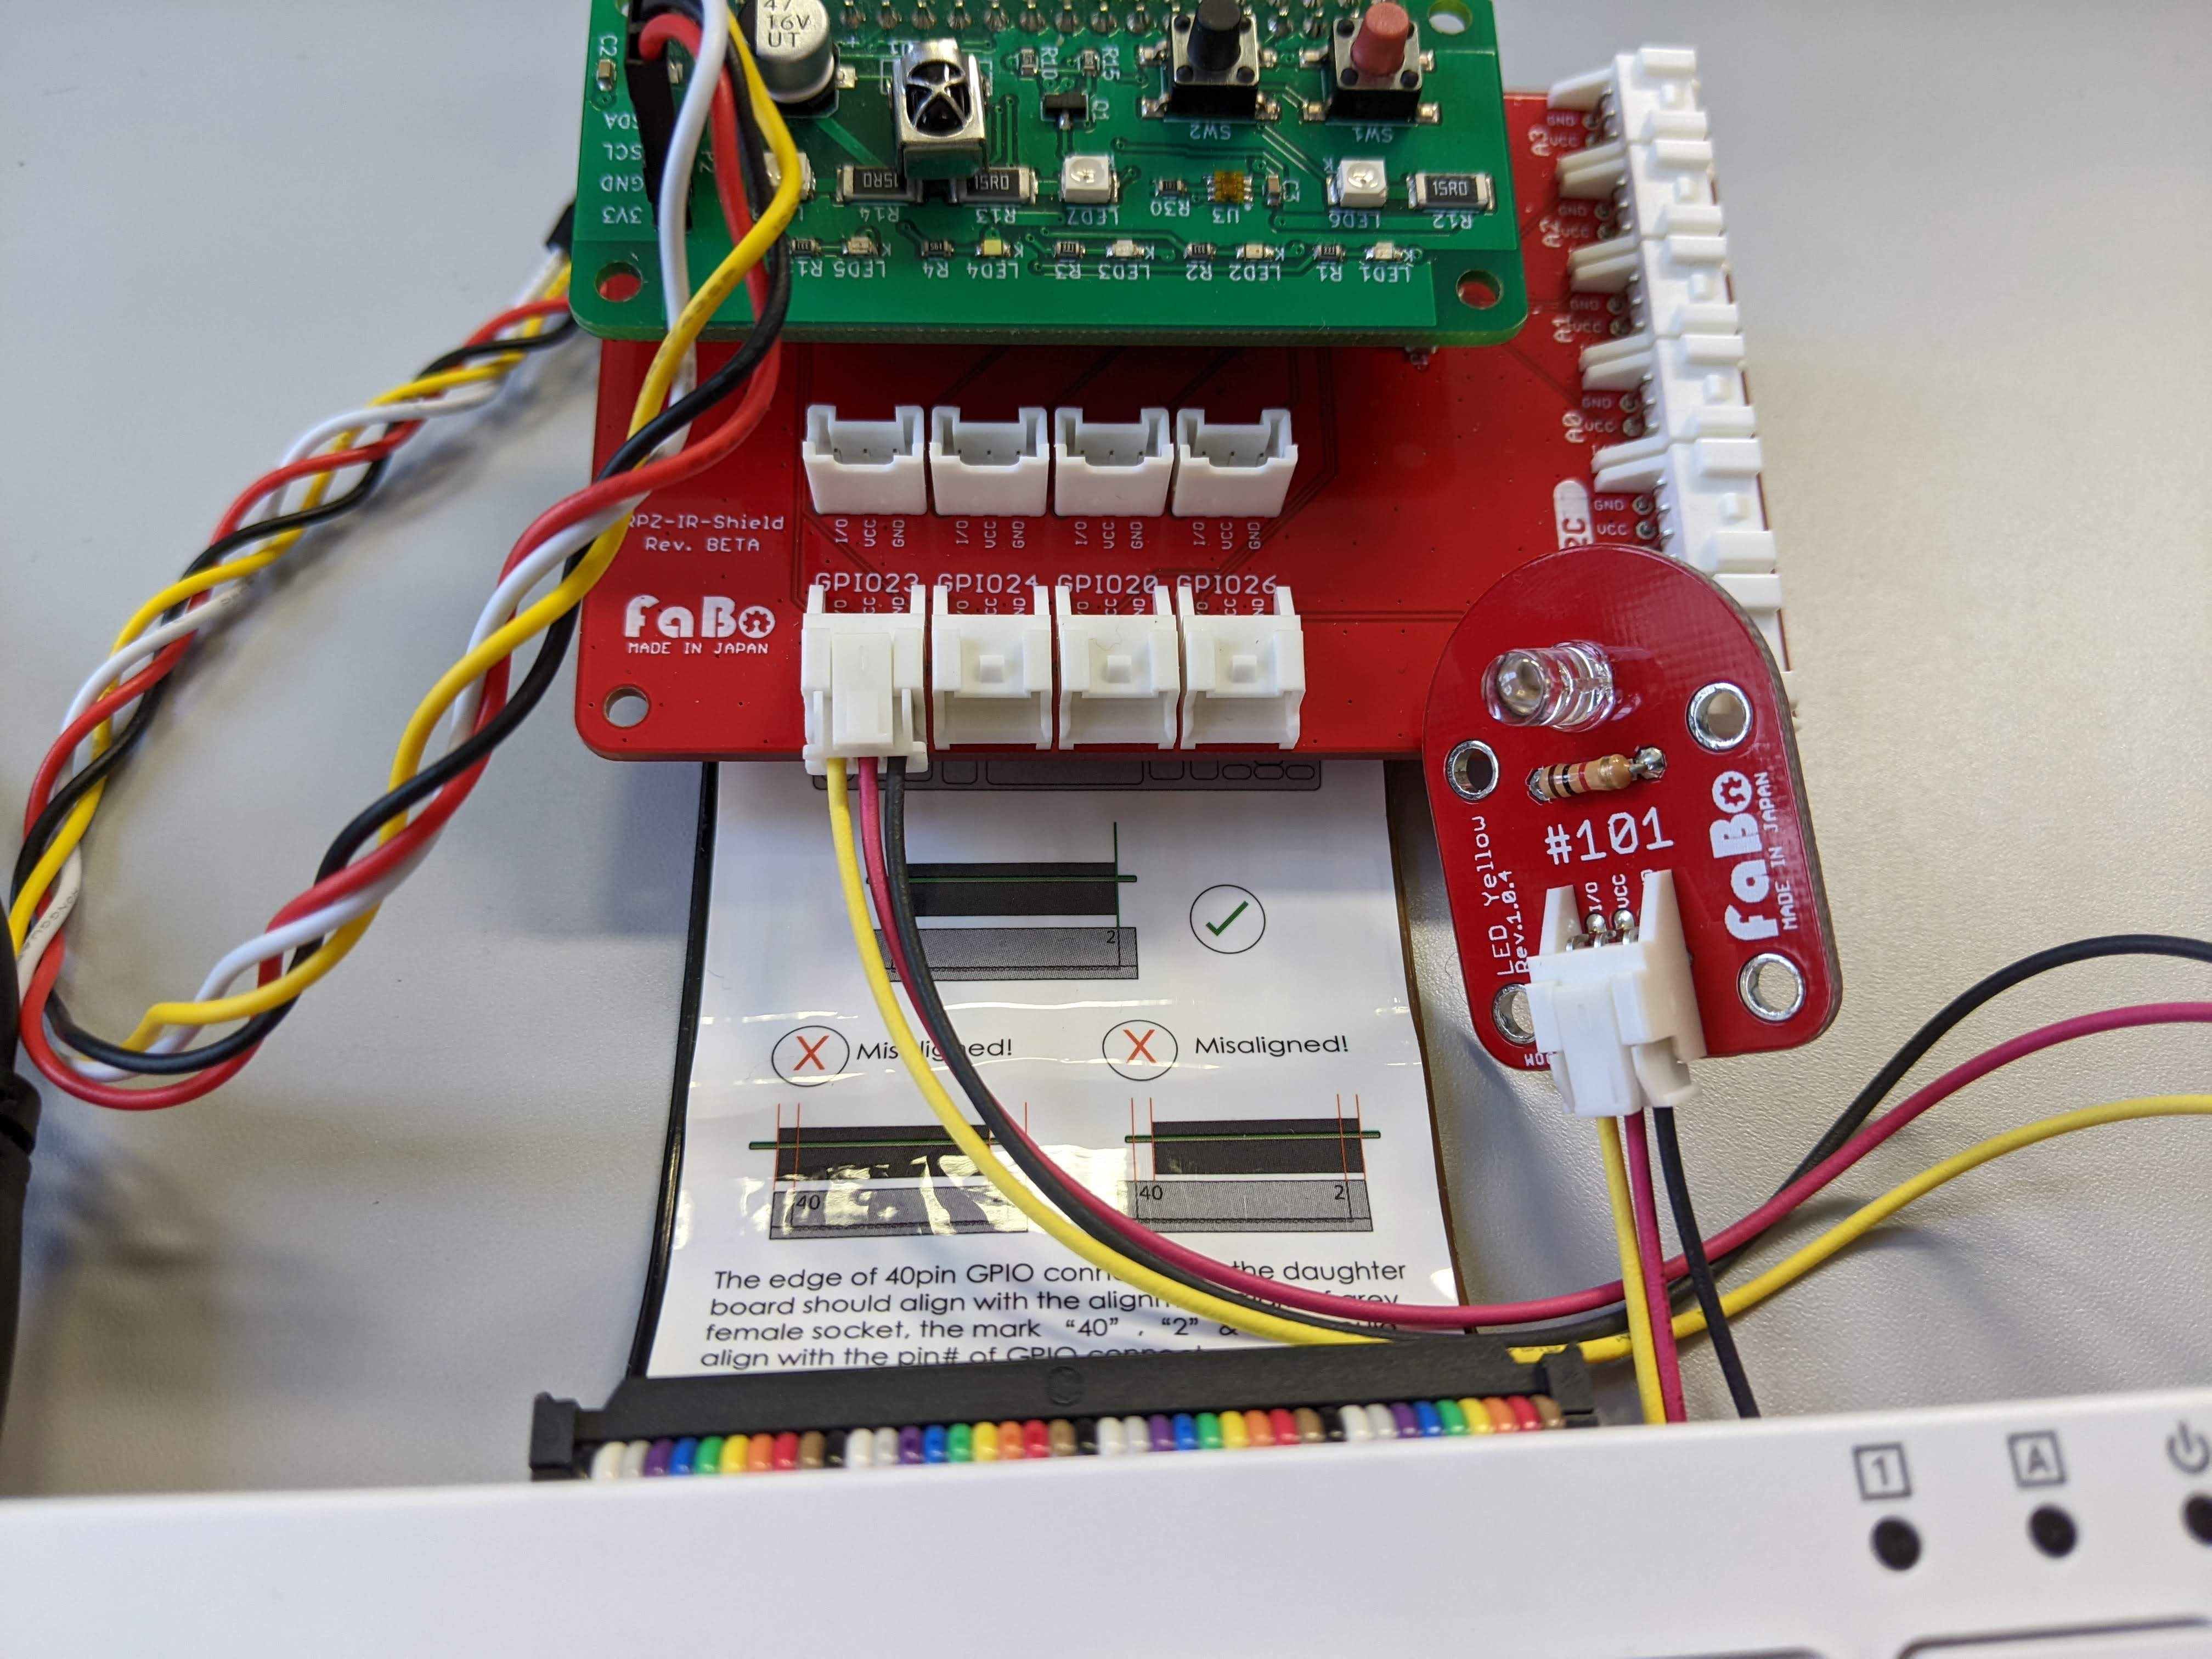
\includegraphics[width=\hsize/2]{images/chap05/led_brk_on_fabo_with_sb_zoomed.jpg}
%     \caption{シールドとケーブルの接続}
%   \end{figure}
%   \item ケーブルを外す時は、とがっているツメの部分を押して引き抜いてください。抜けない時や分からない時は周りの先生に聞いてみましょう。\\
%   \begin{figure}[H]
%     \begin{minipage}[t]{0.48\columnwidth}
%       \centering
%       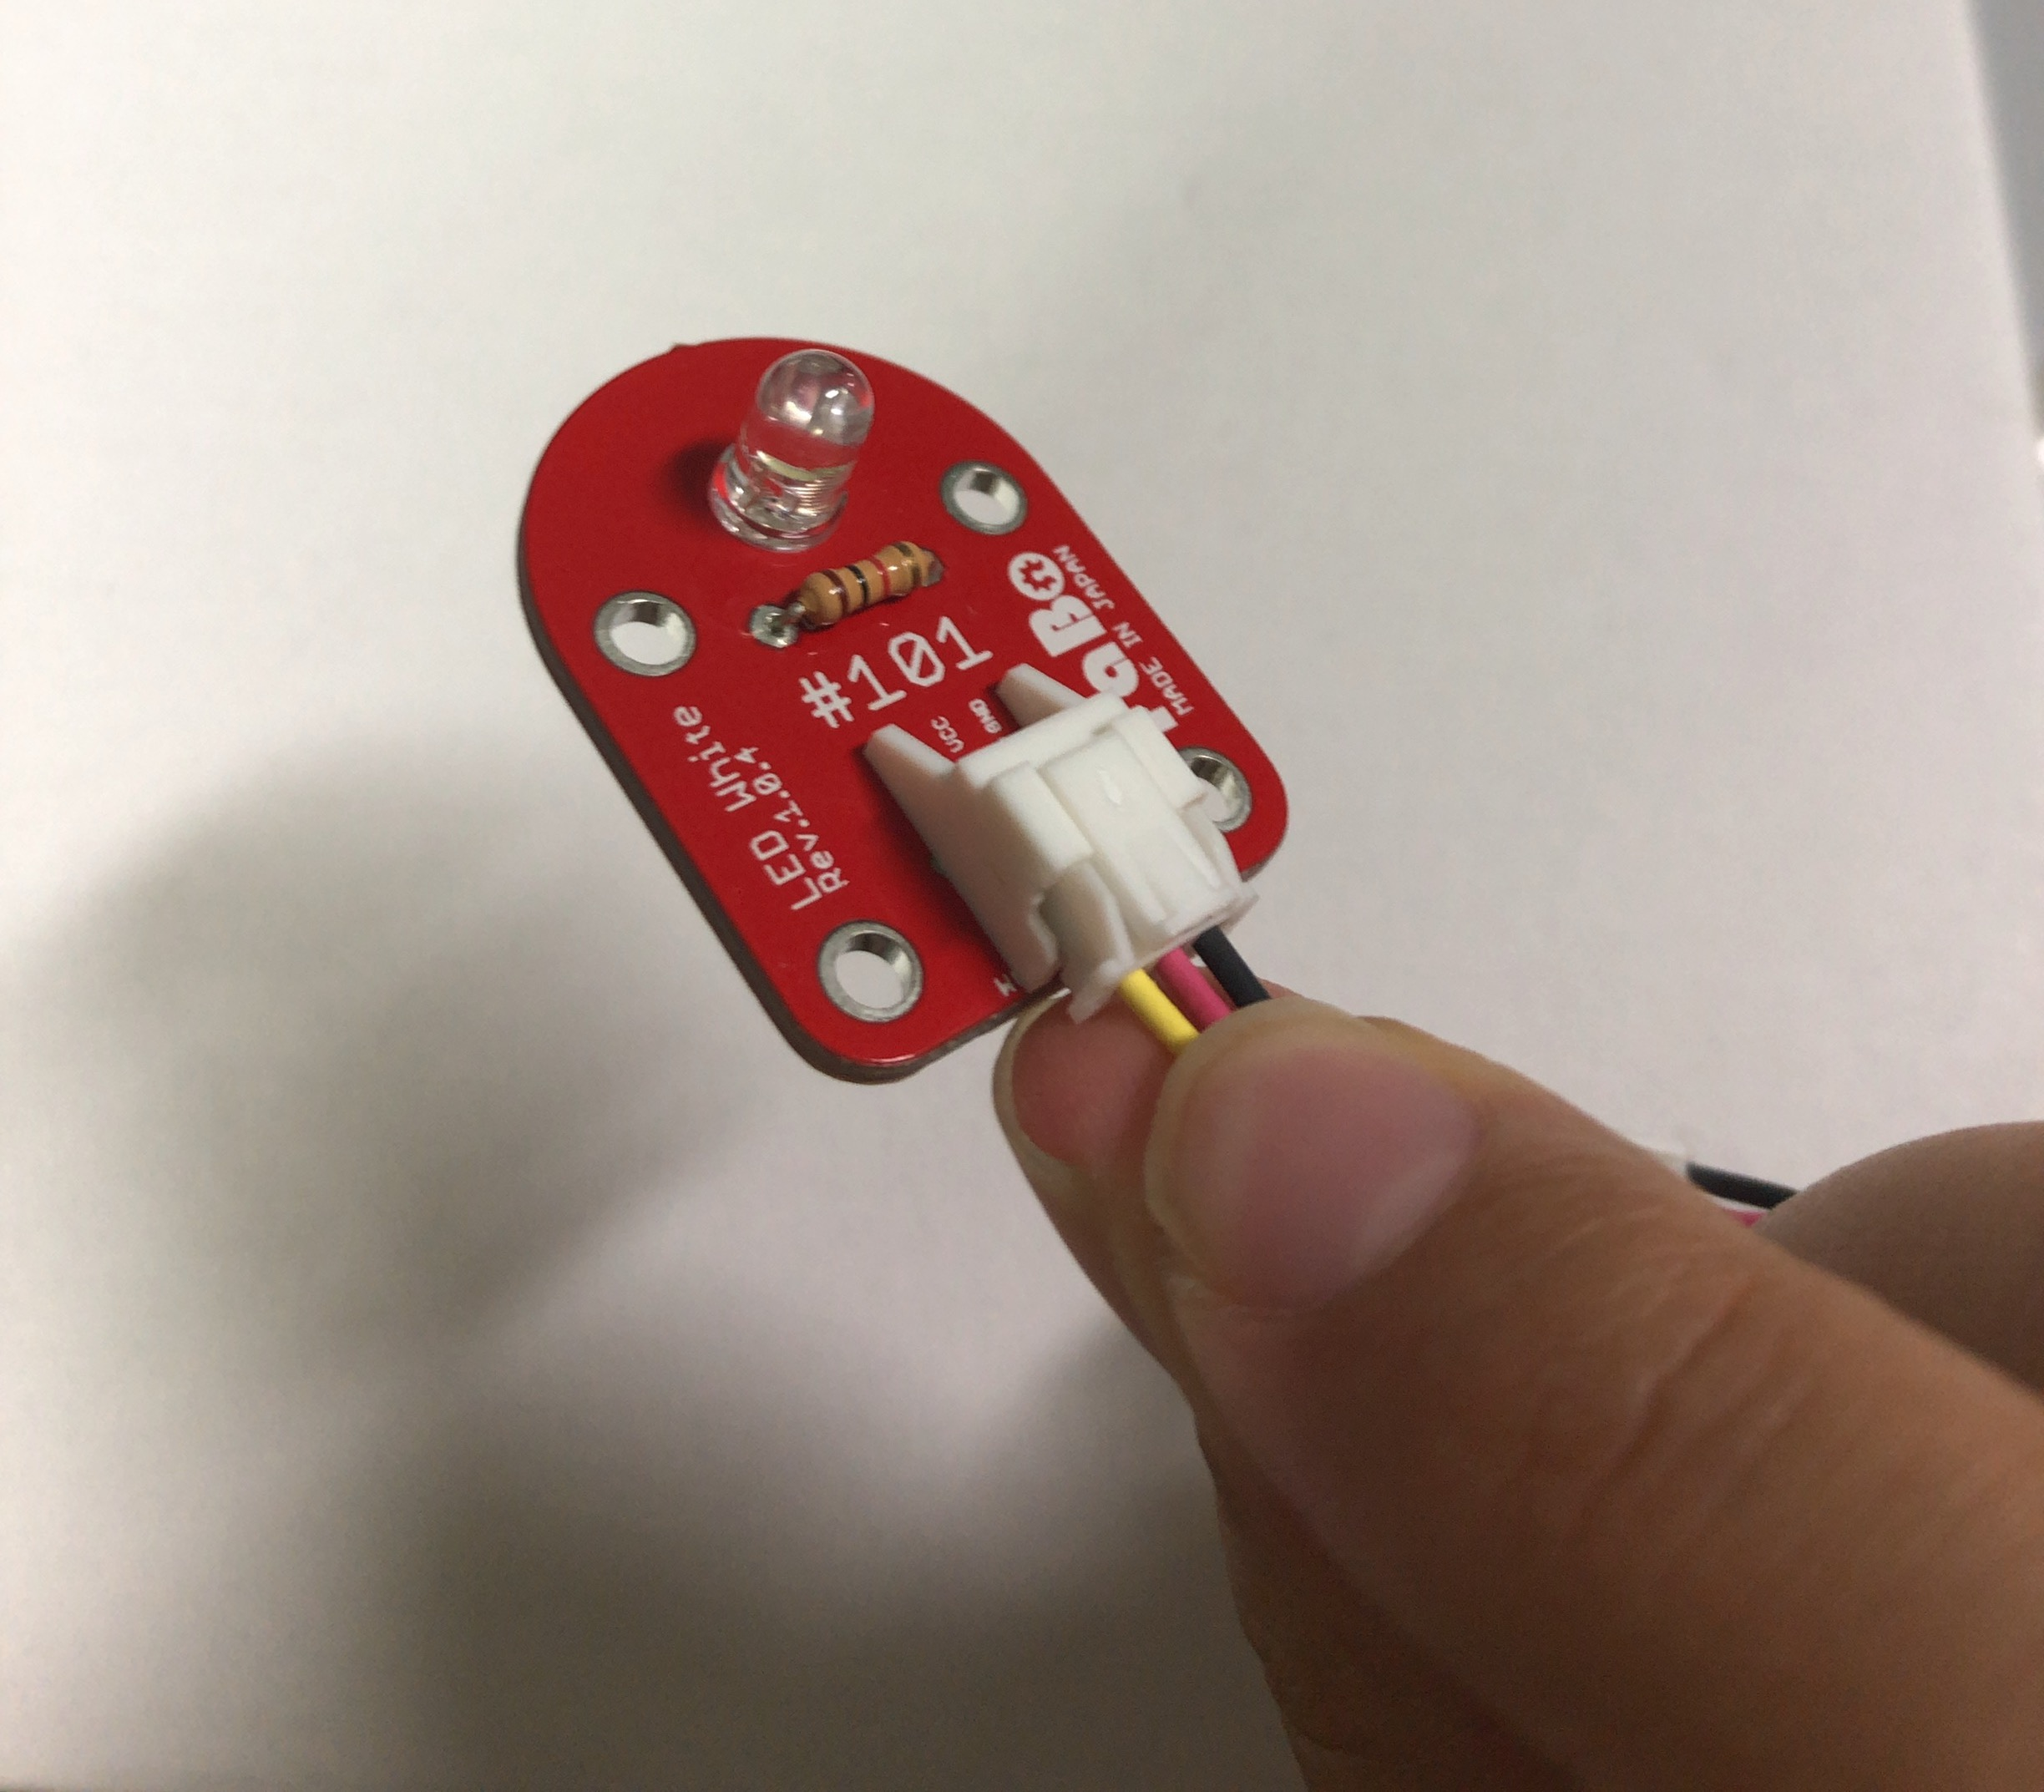
\includegraphics[width=0.8\hsize]{images/chap05/text05-img010.jpg}
%       \caption{ケーブルのツメ}
%       白い部分の下の方を押します。
%     \end{minipage}
%     \hspace{0.04\columnwidth} % ここで隙間作成
%     \begin{minipage}[t]{0.48\columnwidth}
%       \centering
%       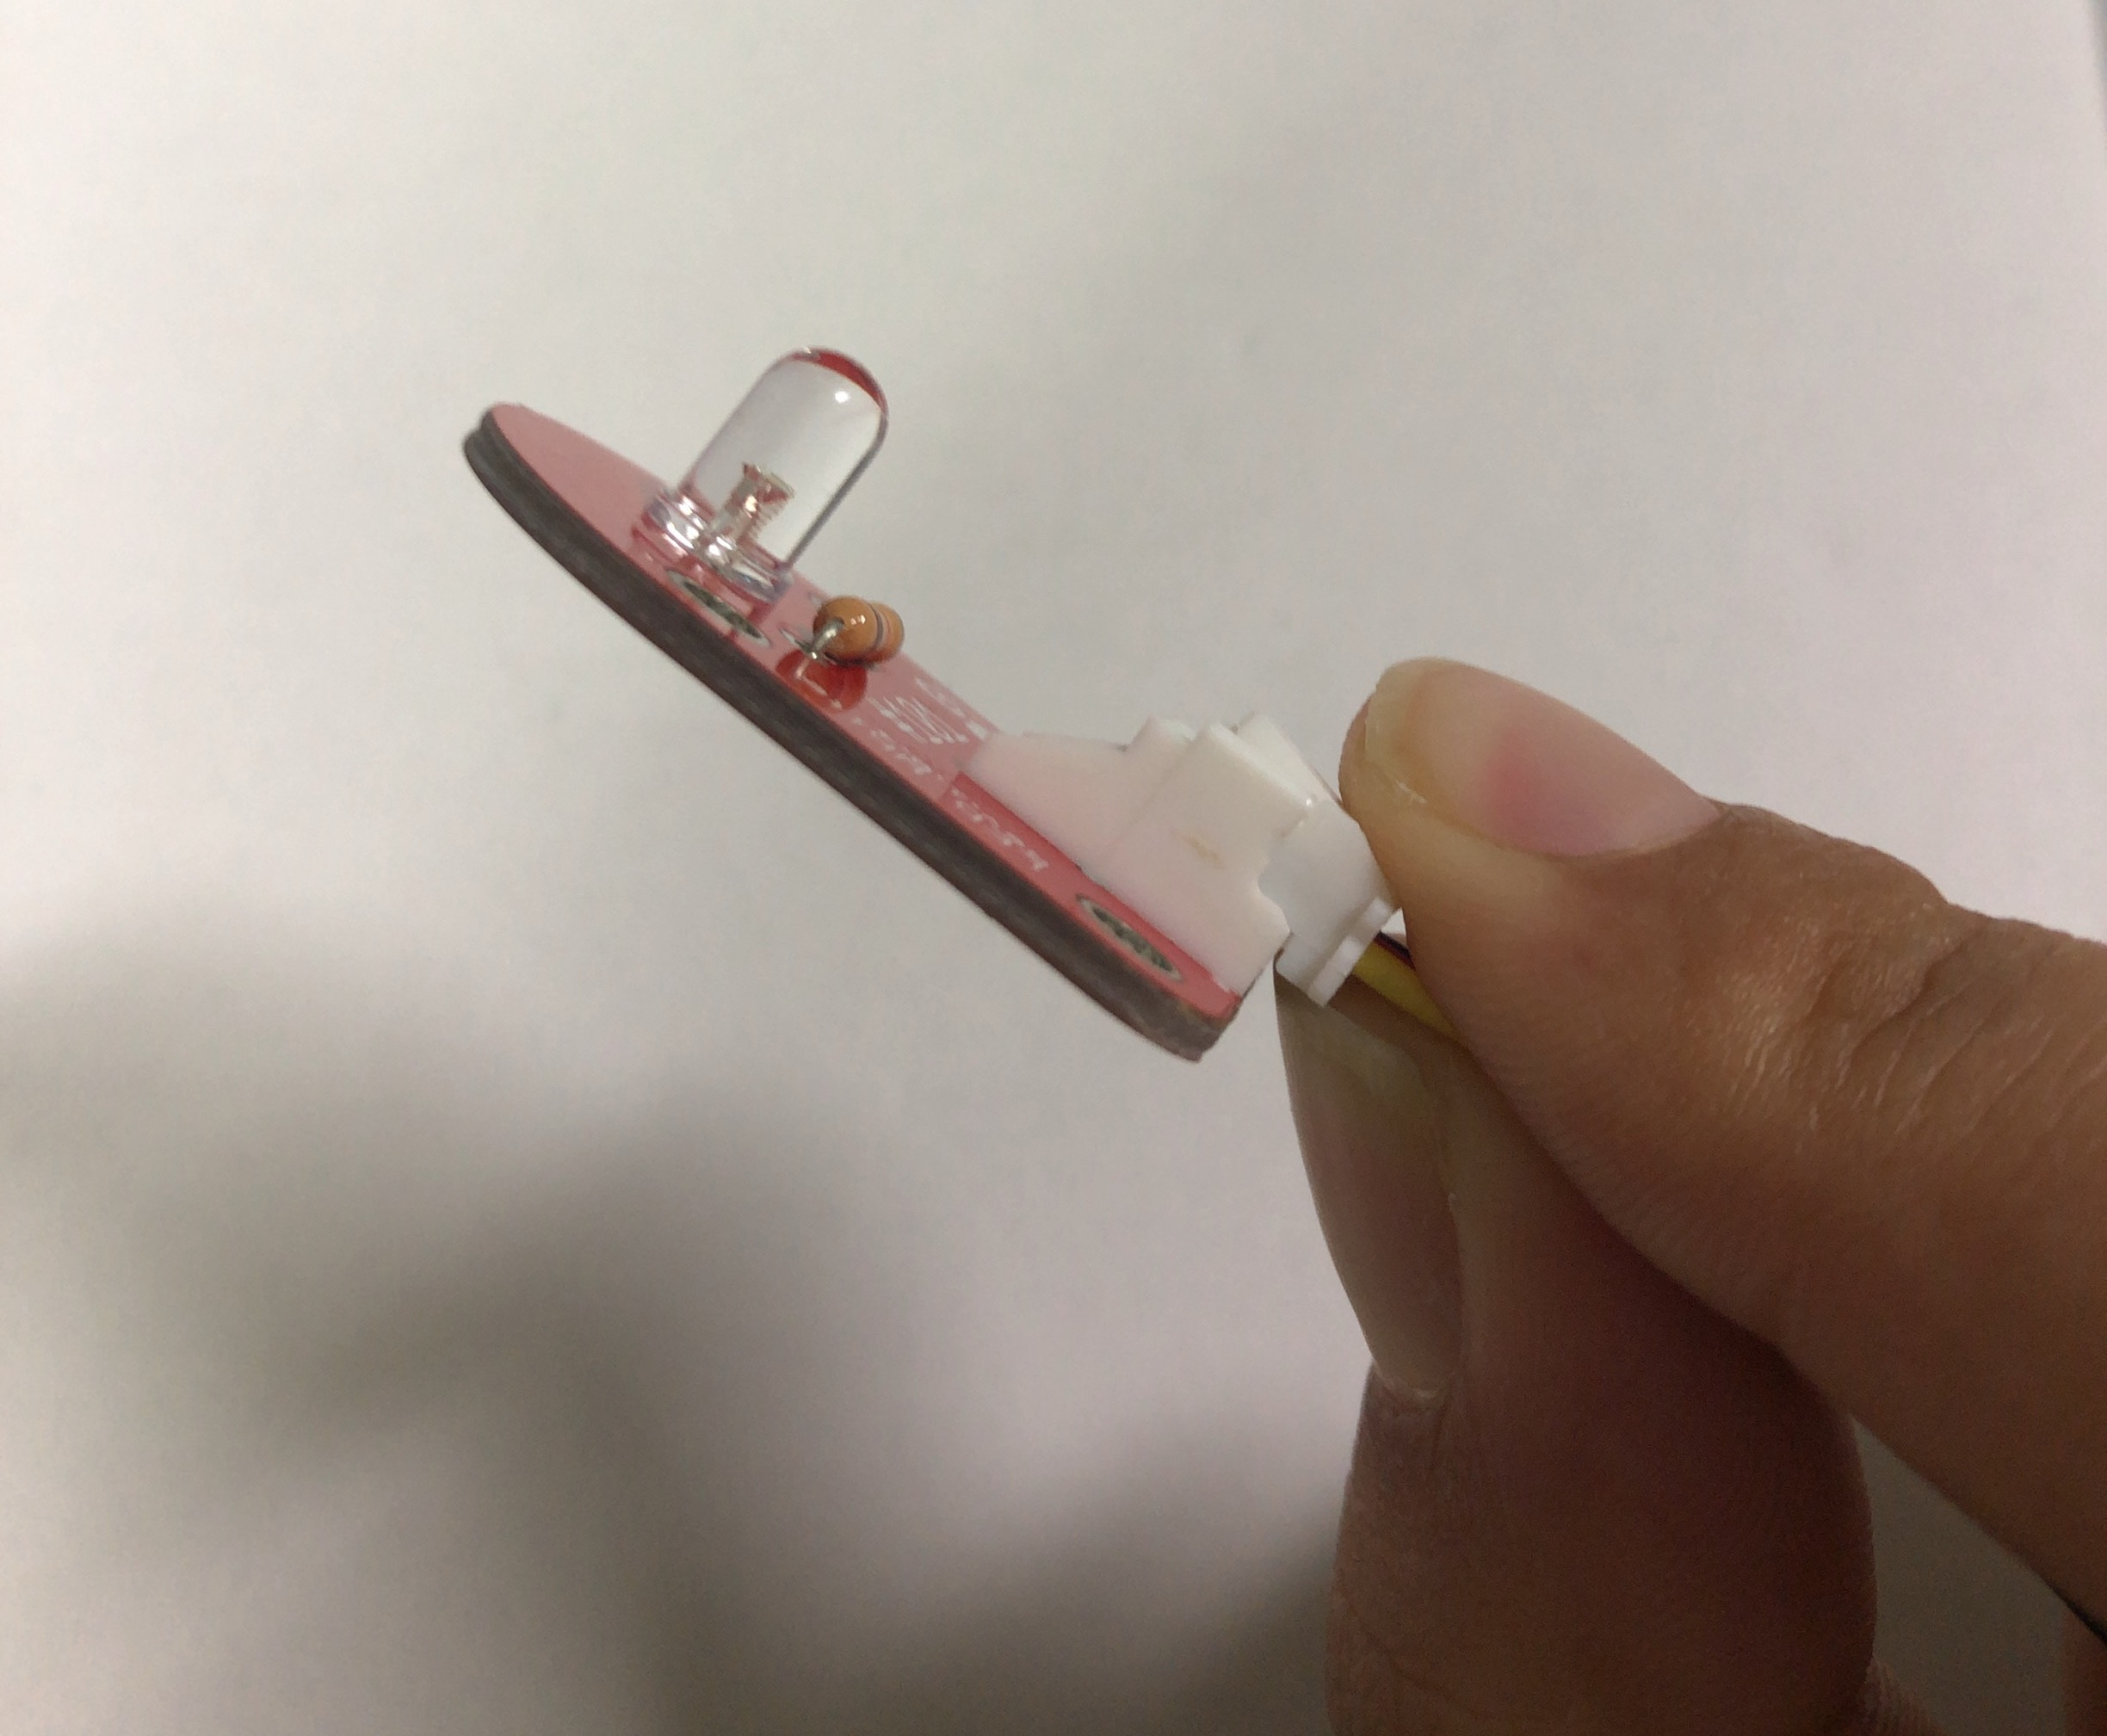
\includegraphics[width=0.8\hsize]{images/chap05/text05-img011.jpg}
%       \caption{ケーブルのツメの押し方}
%       ツメの部分が少し浮いたら引きぬきましょう。抜けないときは無理に引っぱらず、周りの先生に聞きましょう。
%     \end{minipage}
%   \end{figure}
% \end{enumerate}


\begin{tcolorbox}[title=\useOmetoi]
\begin{enumerate}
\addex{Raspberry PiとLEDを上記の手順を見ながらつなげてみましょう。}
\end{enumerate}
\end{tcolorbox}















